\begin{pastexam}[label={px:gk3-099-ds-05}]{高考三級資訊處理 99 年 第五題}
（申論；20 分）

假設有一個陣列 A[0..12]，儲存 13 個數字：4，14，25，31，37，42，56，70，73，83，86，90，94。今使用二元搜尋
（binary search），問：
\begin{itemize}[leftmargin=2.2em]
\item[㈠] 寫出找尋 70 的比較過程（沒寫過程不予計分）。（8 分）
\item[㈡] 列出比較次數最多的所有數字。（6 分）
\item[㈢] 假設現有 100,000 個數字已經依由小而大的次序排列好，請分別使用二元搜尋（binary search）與循序搜尋
（sequential search），計算兩者成功找尋（successful search）的平均比較次數，並說明兩者大概相差多少倍？
（6 分）
\end{itemize}
\end{pastexam}

\begin{pastsoln}
答案：㈠ 依序和 $A[6] = 56$、$A[9] = 83$、$A[7] = 70$ 比，第 $3$ 次找到。 ㈡ 14、31、42、73、86、94（各要比
$4$ 次）。 ㈢ 二元搜尋平均約 $15.7$ 次，循序搜尋平均 $50000.5$ 次，相差約 $3200$ 倍。

採用資結書虛擬碼~17.1 的寫法：$\mathit{low} = 0$、$\mathit{high} = 12$，每次取
$\mathit{mid} = \lfloor (\mathit{low} + \mathit{high})/2 \rfloor$，拿 $A[\mathit{mid}]$ 和要找的 $x$ 比；相等就
找到，$x$ 較大就令 $\mathit{low} = \mathit{mid} + 1$，較小就令 $\mathit{high} = \mathit{mid} - 1$。 「一次比較」
指和一個 $A[\mathit{mid}]$ 比一次（判斷等於、大於或小於算一次）。

\textbf{㈠ 找 $70$。}
\begin{center}
\small
\begin{tabular}{cccccl}
\toprule
第幾次 & low & high & mid & $A[\mathit{mid}]$ & 結果 \\
\midrule
1 & 0 & 12 & 6 & 56 & $70 > 56$，low $\gets 7$ \\
2 & 7 & 12 & 9 & 83 & $70 < 83$，high $\gets 8$ \\
3 & 7 & 8 & 7 & 70 & 相等，找到，在 $A[7]$ \\
\bottomrule
\end{tabular}
\end{center}
共比較 $3$ 次。

\textbf{㈡} 把每個位置第一次被當成 mid 的順序畫成比較樹（節點是索引，括號內是數字）：
\begin{center}
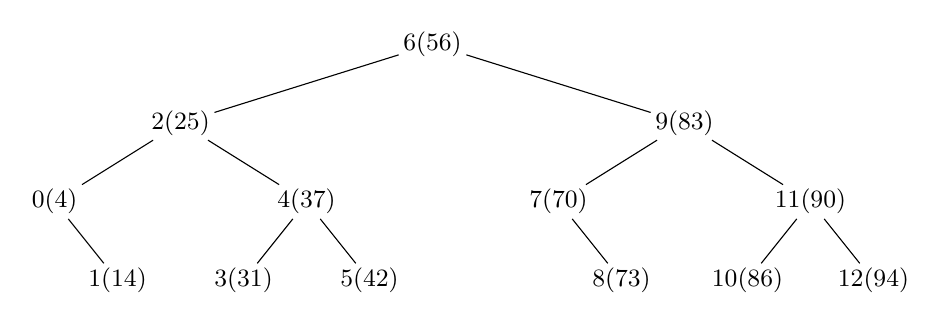
\begin{tikzpicture}[every node/.style={font=\small,inner sep=1.5pt},
  level distance=10mm, level 1/.style={sibling distance=64mm}, level 2/.style={sibling distance=32mm},
  level 3/.style={sibling distance=16mm}]
\node {6(56)}
  child {node {2(25)}
    child {node {0(4)} child[missing] {} child {node {1(14)}}}
    child {node {4(37)} child {node {3(31)}} child {node {5(42)}}}}
  child {node {9(83)}
    child {node {7(70)} child[missing] {} child {node {8(73)}}}
    child {node {11(90)} child {node {10(86)}} child {node {12(94)}}}};
\end{tikzpicture}
\end{center}
找某個數要比的次數＝它在樹中的層數。 第 $1$ 層 $1$ 個（56），第 $2$ 層 $2$ 個（25、83），第 $3$ 層 $4$ 個
（4、37、70、90），第 $4$ 層 $6$ 個。 比較次數最多（$4$ 次）的是 \textbf{14、31、42、73、86、94}。
例如找 $14$：$56 \to 25 \to 4 \to 14$。

\textbf{㈢} $n = 100000$，每個數被找的機率相同。
\begin{itemize}
\item \textbf{循序搜尋}：找第 $i$ 個數要比 $i$ 次，平均
\[
\frac{1 + 2 + \cdots + n}{n} = \frac{n + 1}{2} = 50000.5 \text{ 次}.
\]
\item \textbf{二元搜尋}：比較樹第 $k$ 層最多 $2^{k-1}$ 個節點，前 $16$ 層最多 $2^{16} - 1 = 65535$ 個，
所以第 $1 \sim 16$ 層全滿，剩下 $100000 - 65535 = 34465$ 個在第 $17$ 層。 比較次數總和是
\[
\sum_{k=1}^{16} k \cdot 2^{k-1} + 17 \times 34465 = (15 \cdot 2^{16} + 1) + 585905 = 983041 + 585905 = 1568946,
\]
（用到 $\sum_{k=1}^{h} k \cdot 2^{k-1} = (h - 1)2^h + 1$。）平均
\[
\frac{1568946}{100000} \approx 15.69 \text{ 次},
\]
大約是 $\lg n - 1 \approx 16.6 - 1 = 15.6$。
\item \textbf{倍數}：$50000.5 / 15.69 \approx 3187$，循序搜尋平均大約是二元搜尋的 $3200$ 倍。 一般來說兩者
是 $\Theta(n)$ 對 $\Theta(\log n)$，相差約 $\dfrac{n/2}{\lg n}$ 倍。
\end{itemize}
（第 $17$ 層的 $34465$ 個是比較樹最底層的節點數；二元搜尋的比較樹是「除了最後一層都全滿」的二元樹，資結書
第~17.1~節，所以不論 mid 往下取整或往上取整，總和都一樣。）
\end{pastsoln}
